\section{介绍}
无可否认,我们已经进入了加速计算的时代。 为了满足世界对更多计算的永不满足的需求,
与早期解决方案相比,加速计算通过提供更高的性能和更高的能效来驱动复杂的模拟、人工智能等。

被誉为“计算机架构的新黄金时代”
\footnote{A New Golden Age for Computer Architecture by John L. Hennessy, David A. Patterson; Communications of the ACM, February 2019, Vol. 62 No. 2, Pages 48-60.}
,我们面临着计算设备丰富多样性带来的巨大机遇。 
我们需要不依赖于任何单一供应商或架构的便携式软件开发能力,以便充分发挥加速计算的潜力。

SYCL(发音为sickle)是行业驱动的 Khronos Group 标准,通过 C++ 添加了对数据并行性的高级支持,
以支持加速(异构)系统。 SYCL 为 C++ 编译器提供了利用加速(异构)系统的机制,
与现代 C++ 和 C++ 构建系统高度协同。 SYCL 不是缩写词; SYCL 只是一个名称。

\begin{remark}[加速 vs 异构]
	这些术语是相辅相成的。 异构是一种技术描述,承认以不同方式编程的计算设备的组合。 
	加速是将这种复杂性添加到系统和编程中的动机。 无法保证加速; 
	只有当我们做得正确时,对异构系统进行编程才能加速我们的应用程序。 这本书可以帮助我们教会我们如何正确地做事!
\end{remark}

C++ 中的数据并行性与 SYCL 提供对现代加速(异构)系统中所有计算设备的访问。 
单个 C++ 应用程序可以使用适合当前问题的任意设备组合,包括 GPU、CPU、FPGA 和专用集成电路 (ASIC)。 
没有任何专有的单一供应商解决方案可以为我们提供同等水平的灵活性。

本书教我们如何使用带有 SYCL 的 C++ 进行数据并行编程来利用加速计算,
并提供平衡应用程序性能、跨计算设备的可移植性以及我们作为程序员自己的生产力的实用建议。 
本章通过涵盖包括术语在内的核心概念奠定了基础,当我们学习如何使用数据并行性加速 C++ 程序时,
这些概念对于我们保持新鲜感至关重要。


\subsection{阅读书籍,而不是标准说明书}
没有人愿意被告知“去阅读规范!”——规范很难阅读,SYCL 规范 (www.khronos.org/sycl/) 也不例外。 
就像每一个伟大的语言规范一样,它充满了精确性,但对动机、用法和教学却很淡薄。 本书是使用 SYCL 教授 C++ 的“学习指南”。

没有一本书可以一次性解释所有事情。 因此,本章所做的事情是其他章节所不会做的:代码示例包含一些编程结构,
这些编程结构在后面的章节中才会得到解释。 我们不应该沉迷于完全理解第一章中的编码示例,并相信每一章都会变得更好。

\subsection{SYCL 2020 和 DPC++}
本书使用 SYCL 2020 教授 C++。本书的第一版早于 SYCL 2020 规范,
因此该版本包含的更新包括头文件位置的调整(sycl 而不是 CL)、设备选择器语法以及删除显式主机设备 。

DPC++是一个基于LLVM的开源编译器项目。 我们希望 LLVM 社区最终能够默认支持 SYCL,并且 DPC++ 项目将帮助实现这一目标。 
DPC++ 编译器提供广泛的异构支持,包括 GPU、CPU 和 FPGA。 
本书中的所有示例均适用于 DPC++ 编译器,并且应适用于支持 SYCL 2020 的任何 C++ 编译器。

\begin{remark}
	有关更新的 SYCL 信息(包括任何已知书籍勘误表)的重要资源,
	包括书籍 Github (github.com/Apress/data-parallel-CPP)、
	Khronos Group SYCL 标准网站 (www.khronos.org/sycl) 以及重要的 SYCL教育网站(sycl.tech)。
\end{remark}

截至发布时,尚无 C++ 编译器声称完全符合或符合 SYCL 2020 规范。 
尽管如此,本书中的代码适用于 DPC++ 编译器,并且应该适用于已实现大部分 SYCL 2020 的其他 C++ 编译器。 
我们仅在 SYCL 2020 中使用标准 C++,除了一些特定于 DPC++ 的扩展,
这些扩展在第 17 章(FPGA 编程)、连接到零级后端时的第 20 章(后端互操作性)以及推测未来的尾声中明确指出 。

\subsection{为什么不使用 CUDA?}
与 CUDA 不同,SYCL 支持所有供应商和所有类型的架构(不仅仅是 GPU)的 C++ 数据并行性。 
CUDA 仅专注于 NVIDIA GPU 支持,
其他供应商将其重新用于 GPU 的努力(例如 HIP/ROCm)尽管取得了一些实实在在的成功和实用性,但成功的能力有限。 
随着加速器架构的爆炸式增长,只有 SYCL 能够为我们提供利用这种多样性所需的支持,
并提供多供应商/多架构方法来帮助实现 CUDA 所不提供的可移植性。 
为了更深入地理解这一动机,我们强烈建议阅读(或观看他们精彩演讲的视频录制)行业传奇人物 John L. Hennessy 
和 David A. Patterson 所著的《计算机架构的新黄金时代》。 我们认为这是一篇必读的文章。

第 21 章除了讨论使用 SYCL 将代码从 CUDA 迁移到 C++ 有用的主题之外,对于那些有 CUDA 经验的人来说也很有价值,
可以弥合一些术语和功能差异。 CUDA 之外最重要的功能来自 SYCL 支持多个供应商、
多个架构(不仅仅是 GPU)以及多个后端(甚至同一设备)的能力。 这种灵活性回答了“为什么不使用 CUDA?”的问题。

与 CUDA 或 HIP 相比,SYCL 不涉及任何额外开销。 它不是一个兼容层,而是一种通用方法,无论供应商和架构如何,
都向所有设备开放,同时与现代 C++ 同步。 
与其他开放多供应商和多架构技术(例如 OpenMP 和 OpenCL)一样,最终的证明在于实现,
包括在绝对需要时访问特定于硬件的优化的选项。

\subsection{为什么使用带有 SYCL 的标准 C++?}
正如我们将反复指出的,每个使用 SYCL 的程序首先都是 C++ 程序。 SYCL 不依赖于对 C++ 的任何语言更改。 
SYCL 确实将 C++ 编程带到了没有 SYCL 就无法实现的地方。 
我们毫不怀疑所有用于加速计算的编程将继续影响包括 C++ 在内的语言标准,
但我们不认为 C++ 标准应该(或将)很快发展以取代 SYCL 的需求。 
SYCL 具有一组丰富的功能,我们在本书中将介绍这些功能,这些功能通过类扩展 C++ 以及对新编译器功能的丰富支持,
以满足多供应商和多体系结构支持的需求(目前已经存在)。

\subsection{获取支持 SYCL 的 C++ 编译器}
本书中的所有示例都可以与 DPC++ 编译器的所有不同发行版一起编译和使用,
并且应该与支持 SYCL 的其他 C++ 编译器一起编译(请参阅 www.khronos.org/sycl 上的“SYCL 编译器开发”)。 
我们小心地注意到,在发布时,使用了 DPC++ 特定扩展的极少数地方。

作者推荐 DPC++ 编译器有多种原因,其中包括我们与 DPC++ 编译器的密切联系。 DPC++是一个支持SYCL的开源编译器项目。 
通过使用 LLVM,DPC++ 编译器项目可以访问多种设备的后端。 
这已经导致对 Intel、NVIDIA 和 AMD GPU、众多 CPU 和 Intel FPGA 的支持。 
扩展和增强对多个供应商和多个架构的开放支持的能力使 LLVM 成为支持 SYCL 的开源工作的绝佳选择。

DPC++ 编译器有多个发行版,增加了额外的工具和库,可作为大型项目的一部分提供,
为异构系统提供广泛的支持,其中包括库、调试器和其他工具,称为 oneAPI 项目。 
oneAPI 工具(包括 DPC++ 编译器)可免费获取(www.oneapi.io/implements)。

\subsection{Hello, world! 和 SYCL 程序剖析}

\begin{figure}[H]
	\centering
	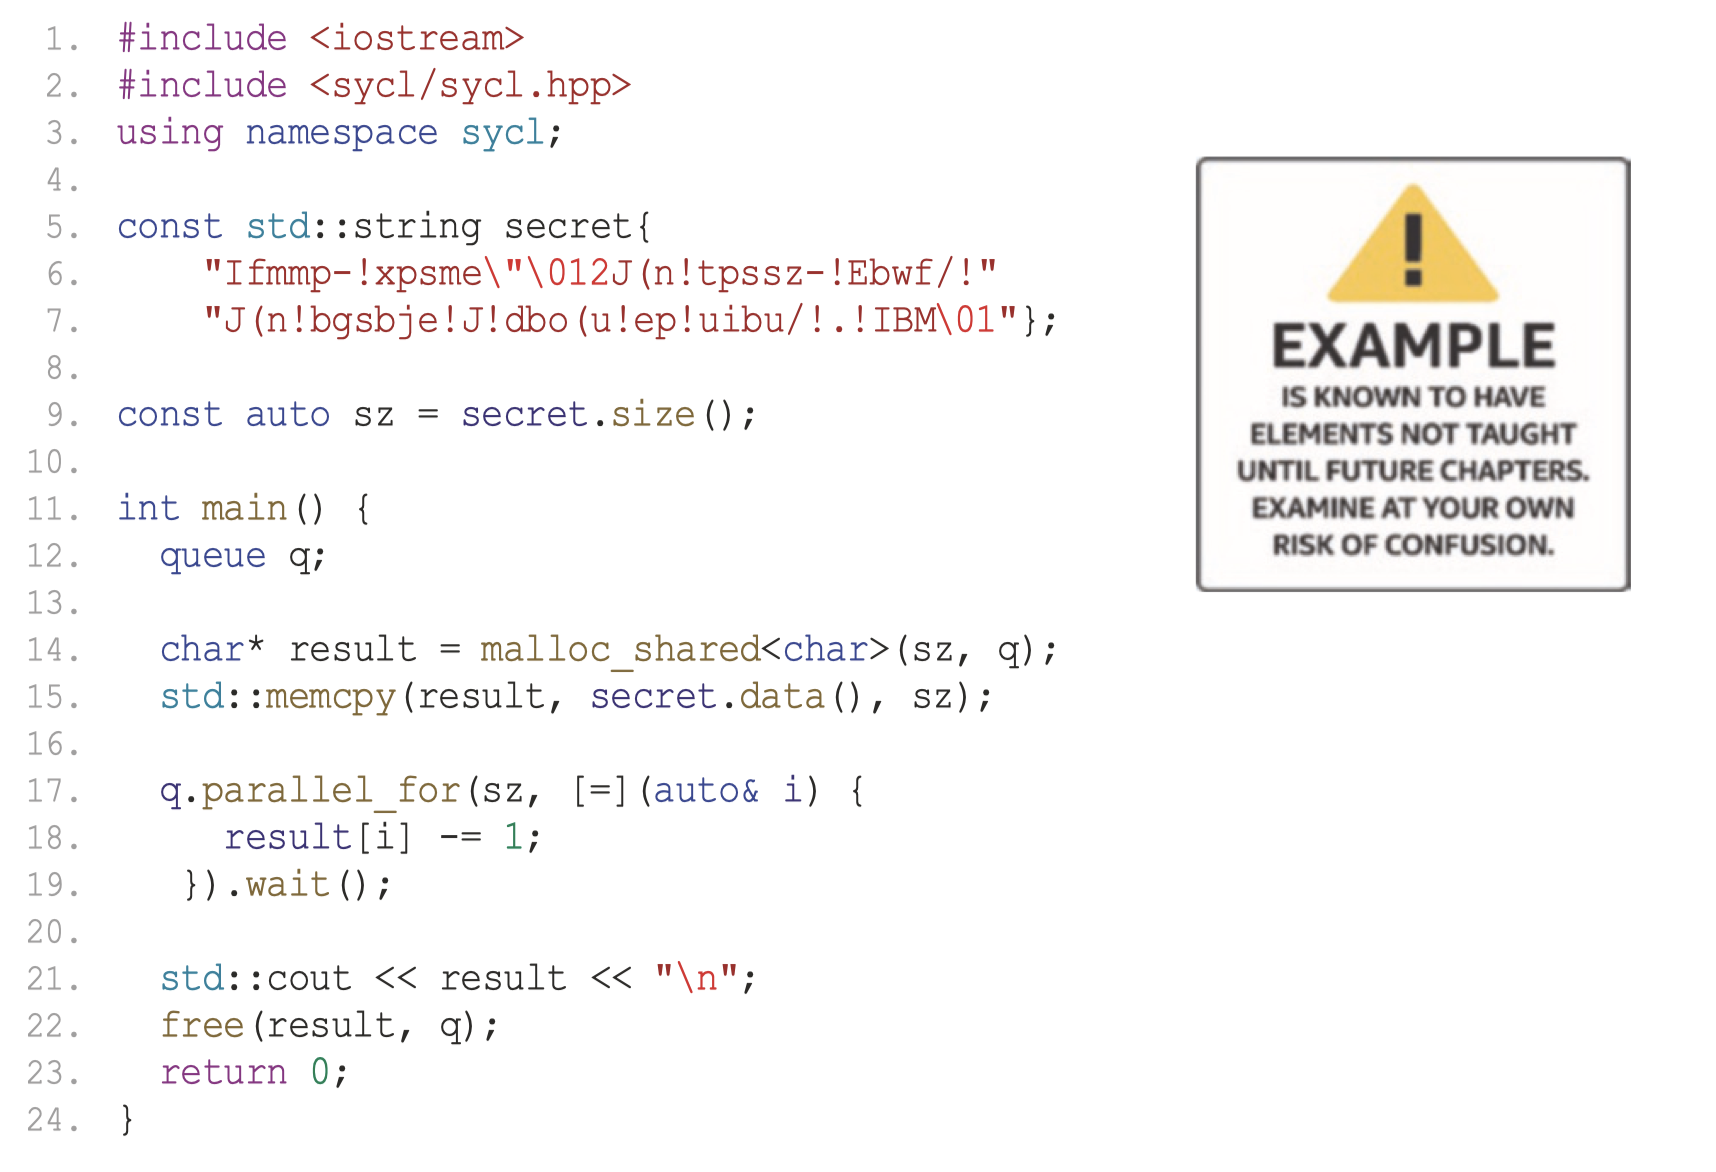
\includegraphics[width=0.9\textwidth]{figs/F1.1.png}
	\caption{\textit{你好数据并行编程。}}
\end{figure}

图 1-1 显示了 SYCL 程序示例。 编译并运行它会打印以下内容:

Hello, world!(以及一些通过运行它来体验的附加文本)

到第 4 章结束时,我们将完全理解这个示例。
在此之前,我们可以观察到定义所有 SYCL 结构所需的 <sycl/sycl.hpp>(第 2 行)的单个包含。 
所有 SYCL 构造都位于名为 sycl 的命名空间内。

\begin{itemize}
	\item 第3 行让我们避免一遍又一遍地编写sycl::。

	\item 第 12 行实例化一个针对特定设备的工作请求队列(第 2 章)。

	\item 第14 行为与设备共享的数据创建分配(第3 章)。

	\item 第15 行将秘密字符串复制到设备内存中,Kernel将在其中对其进行处理。

	\item 第17 行将工作排队到设备(第4 章)。

	\item 第18 行是唯一将在设备上运行的代码行。 所有其他代码都在主机(CPU)上运行。
\end{itemize}

第 18 行是我们要在设备上运行的Kernel代码。 该Kernel代码减少一个字符。 
借助parallel\_for() 的强大功能,该Kernel会在秘密字符串中的每个字符上运行,以便将其解码为结果字符串。 
不需要对工作进行排序,一旦parallel\_for 将工作排队,它就会相对于主程序异步运行。 
在查看结果之前等待(第 19 行)以确保Kernel已完成是至关重要的,
因为在本例中我们使用了一个方便的功能(统一共享内存,第 6 章)。 
如果没有等待,输出可能会在所有字符都被解密之前发生。 还有更多内容需要讨论,但这是后面章节的工作。

\subsection{队列和操作}
第 2 章讨论队列和操作,但现在我们可以从简单的解释开始。 队列是允许应用程序直接在设备上完成工作的唯一连接。 
可以将两种类型的操作放入队列中:(a) 要执行的代码和 (b) 内存操作。 
要执行的代码通过 single\_task 或 parallel\_for 表示(如图 1-1 中使用)。 
内存操作执行主机和设备之间的复制操作或填充操作以初始化内存。 
仅当我们寻求比自动为我们完成的控制更多的控制时,我们才需要使用内存操作。 这些都将在本书后面从第 2 章开始讨论。
现在,我们应该意识到队列是允许我们命令设备的连接,并且我们有一组可用的操作来放入队列以执行代码和移动数据。
了解请求的操作无需等待即可放入队列也非常重要。主机在将操作提交到队列中后,继续执行程序,
而设备最终将异步执行通过队列请求的操作。

\begin{remark}[队列将我们与设备连接起来]
我们将操作提交到队列中以请求计算工作和数据移动。
	
操作异步发生。
\end{remark}


\subsection{一切都与并行性有关}
由于数据并行性的 C++ 编程都是关于并行性的,所以让我们从这个关键概念开始。 
并行编程的目标是更快地计算。 事实证明,这有两个方面:增加吞吐量和减少延迟。

\subsubsection{吞吐量}
当我们在规定的时间内完成更多的工作时,程序的吞吐量就会增加。 像流水线这样的技术可能会延长完成单个工作项所需的时间,
从而允许工作重叠,从而导致单位时间内完成更多的工作。 人类在一起工作时经常会遇到这种情况。 
共享工作本身就涉及协调开销,这通常会减慢完成单个项目的时间。 然而,多人的力量会带来更多的吞吐量。 
计算机也不例外——将工作分散到更多的处理核心会增加每个工作单元的开销,这可能会导致一些延迟,
但目标是完成更多的总工作,因为我们有更多的处理核心一起工作。

\subsubsection{延迟}
如果我们想更快地完成一件事,例如分析语音命令并制定响应,该怎么办? 如果我们只关心吞吐量,响应时间可能会变得难以忍受。 
减少延迟的概念要求我们将一项工作分解为可以并行处理的部分。 
对于吞吐量,图像处理可能会将整个图像分配给不同的处理单元 - 在这种情况下,我们的目标可能是优化每秒的图像。 
对于延迟,图像处理可能会将图像中的每个像素分配给不同的处理核心 - 在这种情况下,
我们的目标可能是最大化单个图像每秒的像素数。

\subsubsection{并行思维}
成功的并行程序员在编程中使用这两种技术。 这是我们寻求并行思考的开始。

我们要调整思路,首先考虑在我们的算法和应用程序中可以在哪里找到并行性。 
我们还考虑了表达并行性的不同方式如何影响我们最终实现的性能。 一下子要考虑的东西太多了。 
对并行思考的追求成为并行程序员的终生旅程。 我们可以在这里学习一些技巧。

\subsubsection{阿姆达尔和古斯塔夫森}
阿姆达尔定律由超级计算机先驱 Gene Amdahl 在 1967 年提出,是一个预测使用多个处理器时理论上最大加速的公式。 
Amdahl 感叹并行性的最大增益仅限于 (1/(1-p)),其中 p 是并行运行的程序的比例。 
如果我们只并行运行三分之二的程序,那么该程序最多可以加速 3 倍。我们绝对需要深入理解这个概念! 
发生这种情况是因为无论我们使三分之二的程序运行得有多快,另外三分之一仍然需要相同的时间才能完成。 
即使我们添加 100 个 GPU,性能也只能提高 3 倍。

多年来,一些人认为这证明并行计算不会取得成果。 
1988 年,约翰·古斯塔夫森 (John Gustafson) 写了一篇题为“重新评估阿姆达尔定律”的文章。 
他观察到并行性并不是用来加速固定工作负载,而是用来扩展工作量。 人类也会经历同样的事情。 
在更多人和卡车的帮助下,一名送货员无法更快地交付单个包裹。 
然而,一百个人和卡车可以比一个司机开一辆卡车运送一百个包裹更快。 
多个驱动程序肯定会增加吞吐量,并且通常还会减少包裹递送的延迟。 
阿姆达尔定律告诉我们,单个司机无法通过增加 99 名拥有自己卡车的司机来更快地交付一个包裹。 
古斯塔夫森注意到,通过这些额外的司机和卡车,可以更快地运送一百个包裹。

这强调了并行性是最有用的,因为我们解决的问题的规模逐年增长。 
如果我们只是想年复一年地更快地运行相同大小的问题,那么并行性的研究就不那么重要了。 
这种对解决越来越大问题的追求激发了我们对利用 C++ 和 SYCL 来开发数据并行性的兴趣,以实现计算机的未来(异构/加速系统)。

\subsubsection{规模效应}
“缩放”这个词出现在我们之前的讨论中。 缩放是衡量当额外的计算可用时程序加速的程度(简称为“加速”)。 
如果一百个包裹与一个包裹同时交付,只需一百辆卡车配备司机而不是单一卡车和司机,就会实现完美的加速。 
当然,这种方式并不可靠。 在某些时候,存在限制加速的瓶颈。 配送中心可能没有一百个卡车停靠点。 
在计算机程序中,瓶颈通常涉及将数据移动到将要处理的位置。 分发到一百辆卡车类似于必须将数据分发到一百个处理核心。 
分配行为不是瞬时的。 第 3 章开始了我们探索如何将数据分发到异构系统中需要的地方的旅程。 
至关重要的是,我们知道数据分发是有成本的,而该成本会影响我们对应用程序的预期扩展程度。

\subsubsection{异构系统}
就我们的目的而言,异构系统是包含多种类型计算设备的任何系统。 
例如,同时具有中央处理单元(CPU)和图形处理单元(GPU)的系统是异构系统。 
CPU 通常简称为处理器,尽管当我们将异构系统中的所有处理单元称为计算处理器时,这可能会令人困惑。 
为了避免这种混淆,SYCL 将处理单元称为设备。 应用程序始终在主机上运行,主机又将工作发送到设备。 
第 2 章开始讨论我们的主应用程序(主机代码)如何将工作(计算)引导到异构系统中的特定设备。

使用带有 SYCL 的 C++ 的程序在主机上运行并向设备发出工作Kernel。 
尽管这可能看起来令人困惑,但重要的是要知道主机通常能够充当设备。 
这有两个关键原因:(1) 主机通常是一个 CPU,如果不存在加速器,
它将运行Kernel - SYCL 对于应用程序可移植性的一个关键承诺是Kernel始终可以在任何系统上运行,
即使是那些系统 没有加速器 - (2) CPU 通常具有矢量、矩阵、张量和/或 AI 处理功能,
这些功能是Kernel可以很好地映射以在其上运行的加速器。

\begin{remark}
	主机代码调用设备上的代码。 主机的功能通常也可以作为设备使用,
	以提供备份设备并提供主机具有的用于处理Kernel的任何加速功能。 我们的主机通常是一个 CPU,
	因此它可以作为 CPU 设备使用。 SYCL 不保证 CPU 设备,仅保证至少有一个设备可作为我们应用程序的默认设备。
\end{remark}

虽然异构从技术角度描述了系统,但使我们的硬件和软件复杂化的原因是为了获得更高的性能。 
因此,加速计算一词在异构系统或其组件的营销中很流行。 我们想强调的是,不能保证加速。 
只有当我们做得正确时,异构系统的编程才会加速我们的应用程序。 这本书可以帮助我们教会我们如何正确地做事!

GPU 已发展成为高性能计算 (HPC) 设备,因此有时被称为通用 GPU 或 GPGPU。 
出于异构编程的目的,我们可以简单地假设我们正在编程如此强大的 GPGPU,并将它们称为 GPU。

如今,异构系统中的设备集合可以包括 CPU、GPU、FPGA(现场可编程门阵列)、DSP(数字信号处理器)、
ASIC(专用集成电路)和 AI 芯片(图形、神经形态等) .)。

此类设备的设计将涉及计算处理器(多处理器)的重复以及与内存等数据源的增加连接(增加带宽)。 
第一个是多处理,对于提高吞吐量特别有用。 在我们的类比中,这是通过添加额外的司机和卡车来完成的。 
后者,更高的数据带宽,对于减少延迟特别有用。 在我们的类比中,这是通过更多的装货码头来完成的,以使卡车能够并行满载。

拥有多种类型的设备,每种设备具有不同的架构,因此具有不同的特性,导致每种设备的编程和优化需求不同。 
这成为使用 SYCL 进行 C++ 以及本书所教授的大部分内容的动机。

\begin{remark}
	创建 SYCL 是为了解决异构(加速)系统的 C++ 数据并行编程挑战。
\end{remark}

\subsubsection{数据并行编程}

自从本书的标题出现以来,“数据并行编程”这个词就一直挥之不去,无法解释。 
数据并行编程侧重于并行性,可以将其想象为并行操作的一堆数据。 这种焦点的转变就像古斯塔夫森与阿姆达尔的对比。 
我们需要运送一百个包裹(实际上是大量数据),以便将工作分配给一百辆配备司机的卡车。 关键概念归结为我们应该划分什么。 
我们应该处理整个图像还是以较小的图块处理它们或逐像素处理它们? 
我们应该将对象集合作为单个集合还是一组较小的对象分组或逐个对象进行分析?

选择正确的工作分工并将其有效地映射到计算资源上是任何使用带有 SYCL 的 C++ 的并行程序员的责任。 
第 4 章开始了这一讨论,并贯穿本书的其余部分。

\subsection{带有 SYCL 的 C++ 的关键属性}
每个使用 SYCL 的程序首先都是 C++ 程序。 SYCL 不依赖于对 C++ 的任何语言更改。

具有 SYCL 支持的 C++ 编译器将根据 SYCL 规范的内置知识来优化代码,
并实现支持,以便异构编译在传统 C++ 构建系统中“正常工作”。

接下来,我们将用 SYCL 解释 C++ 的关键属性:单源样式、主机、设备、Kernel代码和异步任务图。

\subsubsection{单源}
程序是单源的,这意味着同一个翻译单元 \footnote{我们可以只说“文件”,但这在这里并不完全正确。 
翻译单元是编译器的实际输入,由源文件经过 C 预处理器处理为内联头文件和扩展宏后生成。} 
既包含定义要在设备上执行的计算Kernel的代码,也包含协调这些计算Kernel的执行的主机代码。 
第 2 章首先更详细地介绍此功能。 如果我们愿意,我们仍然可以将程序源分为不同的文件和主机和设备代码的翻译单元,
但关键是我们不必这样做!

\subsubsection{主机}
每个程序都是从在主机上运行开始的,程序中的大部分代码行通常都是针对主机的。 
到目前为止,主机一直是CPU。 标准没有这样的要求,所以我们小心地将其描述为主机。 
这似乎不可能是 CPU 以外的任何东西,因为主机需要完全支持 C++17 才能支持所有具有 SYCL 程序的 C++。 
正如我们稍后将看到的,设备(加速器)不需要支持所有 C++17。

\subsubsection{设备}
在一个程序中使用多个设备使得异构编程成为可能。 这就是为什么自从几页前解释异构系统以来,设备这个词在本章中不断出现。 
我们已经了解到,异构系统中的设备集合可以包括GPU、FPGA、DSP、ASIC、CPU和AI芯片,但不限于任何固定列表。

设备是获得加速的目标。 卸载计算的想法是将工作转移到可以加速工作完成的设备。 
我们必须担心如何弥补移动数据所损失的时间——这是一个需要时刻牢记在心的话题。

\subsubsection{Kernel代码}
在具有设备(例如 GPU)的系统上,我们可以设想运行两个或多个程序并希望使用单个设备。 
它们不需要是使用 SYCL 的程序。 如果另一个程序当前正在使用该设备,则程序在设备处理过程中可能会出现延迟。 
这实际上与一般 CPU 的 C++ 程序中使用的原理相同。 
如果我们的 CPU 上同时运行太多活动程序(邮件、浏览器、病毒扫描、视频编辑、照片编辑等),任何系统都可能超载。

在超级计算机上,当节点(CPU + 所有连接的设备)被专门授予单个应用程序时,共享通常不是问题。 
在非超级计算机系统上,我们可以注意到,如果有多个应用程序同时使用相同的设备,程序的性能可能会受到影响。

一切仍然有效,并且我们不需要进行不同的编程。

\subsubsection{异步执行}
设备的代码被指定为Kernel。 这个概念并不是带有 SYCL 的 C++ 独有的:
它是其他卸载加速语言(包括 OpenCL 和 CUDA)的核心概念。 
虽然它与面向循环的方法(例如通常与 OpenMP 目标卸载一起使用)不同,
但它可能类似于最内层循环中的代码主体,而不需要程序员显式编写循环嵌套。

Kernel代码具有某些限制,以允许更广泛的设备支持和大规模并行性。 
Kernel代码不支持的功能列表包括动态多态性、动态内存分配(因此不使用 new 或 delete 运算符进行对象管理)、
静态变量、函数指针、运行时类型信息 (RTTI) 和异常处理。 不允许从Kernel代码调用任何虚拟成员函数和可变参数函数。 
Kernel代码中不允许递归。

\begin{remark}[虚函数]
	虽然我们不会在本书中进一步讨论它,
	但 DPC++ 编译器项目确实有一个实验性扩展(当然,在开源项目中可见)来实现对Kernel中虚拟函数的一些支持。 
	由于有效卸载到加速器的性质,如果没有一些限制,虚函数就无法得到很好的支持,
	但许多用户表示有兴趣看到 SYCL 即使有一些限制也能提供这种支持。 
	开源和开放 SYCL 规范的美妙之处在于有机会参与可以为 C++ 和 SYCL 规范的未来提供信息的实验。 
	请访问 DPC++ 项目 (github.com/intel/llvm) 了解更多信息。
\end{remark}

第 3 章描述了在调用Kernel之前和之后如何完成内存分配,从而确保Kernel始终专注于大规模并行计算。 
第 5 章描述了与设备相关的异常的处理。

C++ 的其余部分在Kernel中是公平的游戏,包括Functor、lambda 表达式、运算符重载、模板、类和静态多态性。 
我们还可以与主机共享数据(参见第 3 章)并共享(非全局)主机变量的只读值(通过 lambda 表达式捕获)。

\textbf{Kernel:矢量加法 (DAXPY)}

\begin{figure}[H]
	\centering
	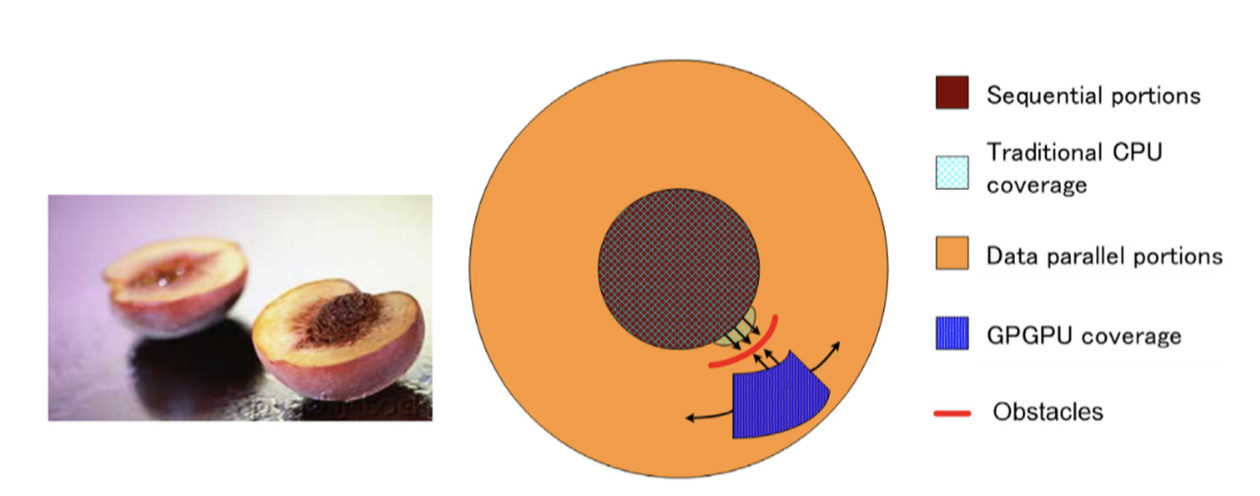
\includegraphics[width=0.9\textwidth]{figs/F1.2.png}
	\caption{\textit{Fortran、C/C++ 和 SYCL 中的 DAXPY 计算。}}
\end{figure}

对于任何处理过计算复杂代码的程序员来说,Kernel都应该感到熟悉。 
考虑实施 DAXPY,它代表“双精度 A 乘以 X 加 Y”。 是几十年来的经典例子。 
图 1-2 显示了用现代 Fortran、C/C++ 和 SYCL 实现的 DAXPY。 
令人惊讶的是,计算线(第 3 行)实际上是相同的。 第 4 章和第 10 章详细解释了Kernel。 
图 1-2 应该有助于消除人们对Kernel难以理解的担忧——即使这些术语对我们来说是新的,它们也应该感到熟悉。

\textbf{异步执行}

使用 C++ 和 SYCL 进行编程的异步特性不容忽视。 理解异步编程至关重要,
原因有两个:(1) 正确使用可以为我们提供更好的性能(更好的扩展),(2) 错误会导致并行编程错误(通常是竞争条件),
从而使我们的应用程序变得不可靠。

异步特性的产生是因为工作是通过请求操作的“队列”传输到设备的。 
主机程序将请求的操作提交到队列中,程序继续执行而不等待任何结果。 
这种无需等待很重要,这样我们就可以尝试让计算资源(设备和主机)始终保持忙碌。 
如果我们必须等待,就会占用主机而不是让主机做有用的工作。 当设备完成时,它还会产生串行瓶颈,直到我们对新工作进行排队。 
正如前面所讨论的,阿姆达尔定律会因为我们花时间而不是并行工作而受到惩罚。 
我们需要构建我们的程序,以便在设备繁忙时将数据移入和移出设备,并在工作可用时保持设备和主机的所有计算能力繁忙。 
如果不这样做,我们就会受到阿姆达尔定律的全面诅咒。

第 3 章开始讨论将我们的程序视为异步任务图,第 8 章极大地扩展了这个概念。

\subsubsection{当我们犯错误时的竞争条件}

\begin{figure}[H]
	\centering
	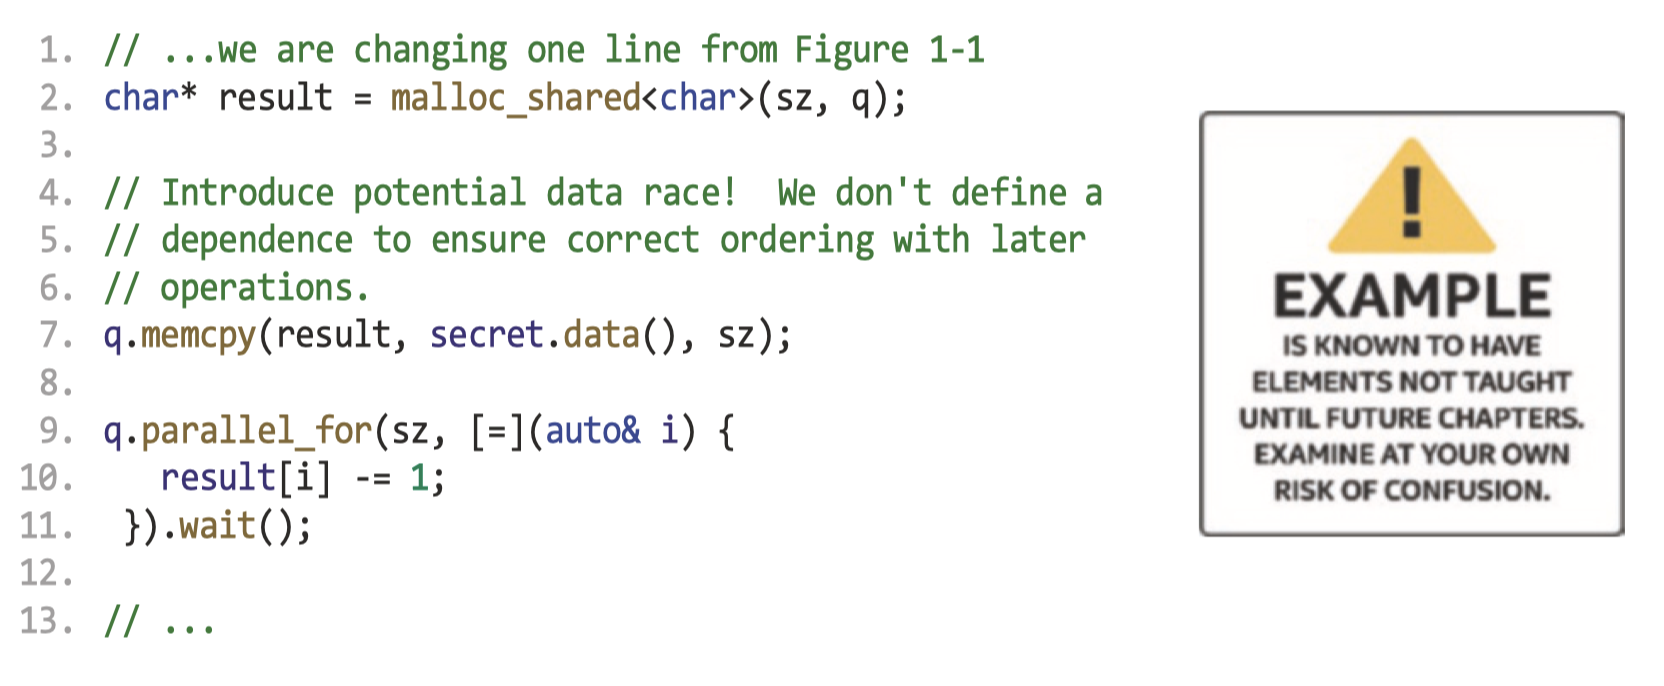
\includegraphics[width=0.9\textwidth]{figs/F1.3.png}
	\caption{\textit{添加竞争条件来说明异步的要点。}}
\end{figure}

在我们的第一个代码示例(图 1-1)中,我们专门在第 19 行执行了“等待”,以防止第 21 行在结果可用之前写出结果中的值。 
我们必须牢记这种异步行为。 在同一代码示例中还做了另一件微妙的事情 - 第 15 行使用 std::memcpy 来加载输入。 
由于 std::memcpy 在主机上运行,因此第 17 行及后续行在第 15 行完成之前不会执行。 
读完第 3 章后,我们可能会想将其更改为使用 q.memcpy(使用 SYCL)。 
我们已经在图 1-3 的第 7 行中做到了这一点。由于这是一个队列提交,因此无法保证它将在第 9 行之前执行。
这会产生竞争条件,这是一种并行编程错误。 当程序的两个部分在没有协调的情况下访问相同的数据时,就会出现竞争条件。 
由于我们希望使用第 7 行写入数据,然后在第 9 行中读取数据,因此我们不希望在第 7 行完成之前执行第 9 行! 
这样的竞争条件将使我们的程序变得不可预测——我们的程序可能会在不同的运行和不同的系统上得到不同的结果。 
解决此问题的方法是在第 7 行末尾添加 .wait() 来显式等待 q.memcpy 完成,然后再继续。这不是最佳解决方案。 
我们可以使用事件依赖来解决这个问题(第 8 章)。 
将队列创建为有序队列还会在 memcpy 和 parallel\_for 之间添加隐式依赖关系。 
作为替代方案,在第 7 章中,我们将看到如何使用缓冲区和访问器编程风格来让 SYCL 管理依赖性并自动等待我们。

\begin{remark}[竞争条件并不总是导致程序失败]
	一位精明的读者注意到,图 1-3 中的代码在他们尝试过的每个系统上都没有失败。 
	使用带有 partition\_max\_sub\_devices==0 的Gpu并没有失败,因为它是一个小型Gpu,
	在memcpy完成之前无法运行parallel\_for。 不管怎样,代码是有缺陷的,因为竞争条件存在,
	即使它不会普遍导致运行时失败。 我们称之为一场竞赛——有时我们赢,有时我们输。 
	此类编码缺陷可能会一直处于休眠状态,直到编译和运行时环境的正确组合导致可观察到的故障为止。
\end{remark}

添加 wait() 会强制 memcpy 和Kernel之间的主机同步,这违背了之前保持设备始终忙碌的建议。 
本书的大部分内容涵盖了不同的选项和权衡,以平衡程序的简单性和系统的有效使用。

\begin{remark}[无序队列 VS 有序队列]
	我们将在本书中使用无序队列,因为它们具有潜在的性能优势,但重要的是要知道对有序队列的支持确实存在。 
	In-order 只是我们在创建队列时可以请求的一个属性。 Cuda 程序员会知道 Cuda 流是无条件有序的。 
	相反,SYCL 队列默认是无序的,
	但可以选择在创建 SYCL 队列时通过传递 in\_order 队列属性来按顺序排列(请参阅第 8 章)。 
	第 21 章为使用 Cuda 的程序员提供了有关此问题和其他注意事项的信息。
\end{remark}

为了帮助检测程序(包括Kernel)中的数据竞争条件,
Intel Inspector(可与前面“获取 DPC++ 编译器”中提到的 oneAPI 工具一起使用)等工具可能会有所帮助。 
此类工具使用的复杂方法通常不适用于所有设备。 检测竞争条件的最佳方法可能是让所有Kernel在 CPU 上运行,
这可以在开发工作期间作为调试技术来完成。 这个调试技巧在第 2 章中作为 Method\#2 进行了讨论。

\begin{remark}[为了教授死锁的概念,哲学家就餐问题是计算机科学中同步问题的经典例证]
想象一下一群哲学家围坐在一张圆桌旁,每个哲学家之间放着一根筷子。 
每个哲学家吃饭时都需要两根筷子,而且他们总是一次拿起一根筷子。 
遗憾的是,如果所有哲学家都先抓住左边的筷子,然后拿着它等待右边的筷子,那么如果他们同时饿了,我们就会遇到问题。 
具体来说,他们最终都会等待一根永远不会可用的筷子。

在这种情况下,糟糕的算法设计(向左抓取,然后等到向右抓取)可能会导致死锁,所有哲学家都饿死。 
那是可悲的。 讨论设计一种算法的多种方法,该算法可以让更少的哲学家饿死,
或者希望是公平的并养活所有人(没有人挨饿),这是一个值得思考的有趣话题,并且已经被写了很多次。

认识到犯此类编程错误是多么容易,在调试时查找它们,并了解如何避免它们,
这些都是成为有效的并行程序员的过程中必不可少的经验。
\end{remark}

\subsubsection{死锁}
死锁是不好的,我们将强调理解并发与并行(参见本章最后一节)对于理解如何避免死锁至关重要。

当两个或多个操作(进程、线程、Kernel等)被阻塞,每个操作都等待另一个操作释放资源或完成任务,从而导致停滞时,就会发生死锁。 
换句话说,我们的应用程序永远不会完成。 每次我们使用等待、同步或锁时,都可能会造成死锁。 
缺乏同步可能会导致死锁,但更常见的是它表现为竞争条件(请参阅上一节)。

死锁可能很难调试。 我们将在本章末尾的“并发与并行”部分重新讨论这一点。

\begin{remark}
	第 4 章将告诉我们“lambda 表达式不被认为是有害的”。 
	我们应该熟悉 lambda 表达式,以便很好地使用 DPC++、SYCL 和现代 C++。
\end{remark}

\subsubsection{C++ Lambda 表达式}
现代 C++ 的一个被并行编程技术大量使用的功能是 lambda 表达式。 
Kernel(在设备上运行的代码)可以用多种方式表达,最常见的一种是 lambda 表达式。 
第 10 章讨论了Kernel可以采用的所有各种形式,包括 lambda 表达式。 
在这里,我们回顾了 C++ lambda 表达式以及有关用于定义Kernel的一些注释。 
在我们在中间的章节中了解了有关 SYCL 的更多信息之后,第 10 章将扩展Kernel方面的内容。

图 1-3 中的代码有一个 lambda 表达式。 我们可以看到它,因为它以非常明确的 [=] 开头。 
在 C++ 中,lambda 以方括号开头,右方括号之前的信息表示如何捕获 lambda 中使用但未作为参数显式传递给它的变量。 
对于 SYCL 中的Kernel,捕获必须按值进行,该值通过在括号内包含等号来表示。

C++11 中引入了对 lambda 表达式的支持。 它们用于创建匿名函数对象(尽管我们可以将它们分配给命名变量),
这些对象可以从封闭范围捕获变量。 C++ lambda 表达式的基本语法是

[ capture-list ] ( params ) -> ret { body }


其中

\begin{itemize}
	\item capture-list 是一个以逗号分隔的捕获列表。 我们通过在捕获列表中列出变量名称来按值捕获变量。 
	我们通过在变量前面加上 \& 符号来通过引用捕获变量,例如 \&v。 
	还有一些适用于所有作用域内自动变量的简写:[=] 用于捕获在正文中按值使用的所有自动变量和按引用捕获当前对象,
	[\&] 用于捕获在正文中使用的所有自动变量 body 以及当前对象的引用,并且 [] 不捕获任何内容。 
	对于 SYCL,始终使用 [=],因为不允许通过引用捕获变量以在Kernel中使用。 
	根据 C++ 标准,全局变量不会在 lambda 中捕获。 
	非全局静态变量可以在Kernel中使用,但前提是它们是 const。 
	这里提到的一些限制允许Kernel在不同的设备架构和实现中保持一致的行为。

	\item params 是函数参数的列表,就像命名函数一样。 
	SYCL 提供参数来标识正在调用Kernel来处理的元素:这可以是唯一的 id(一维)或 2D 或 3D id。 
	这些将在第 4 章中讨论。

	\item ret 是返回类型。 如果未指定 ->ret,则从 return 语句推断。
	缺少 return 语句或返回没有值,意味着返回类型为 void。 
	SYCL Kernel必须始终具有 void 的返回类型,因此我们不应该使用此语法来指定Kernel的返回类型。

	\item body 是函数体。 对于 SYCL Kernel,该Kernel的内容有一些限制(请参阅本章前面的“Kernel代码”部分)。
\end{itemize}

\begin{figure}[H]
	\centering
	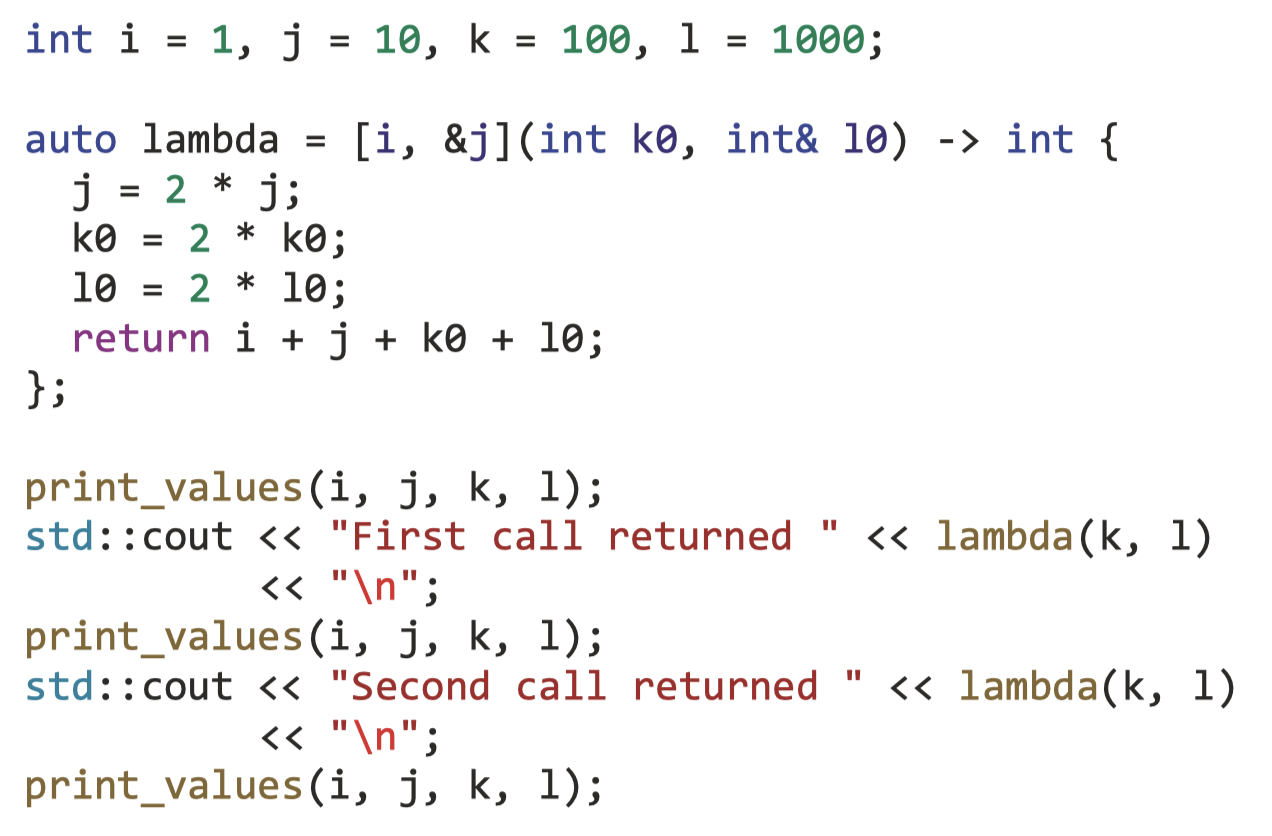
\includegraphics[width=0.9\textwidth]{figs/F1.4.png}
	\caption{\textit{C++ 代码中的 Lambda 表达式。}}
\end{figure}

\begin{figure}[H]
	\centering
	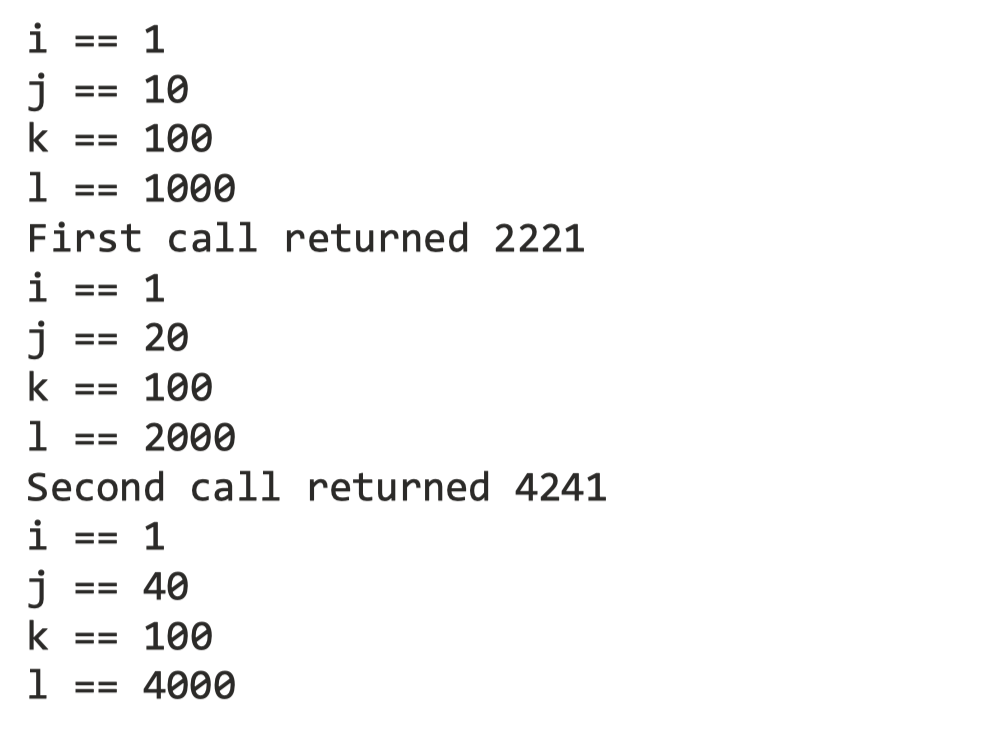
\includegraphics[width=0.9\textwidth]{figs/F1.5.png}
	\caption{\textit{图 1-4 中 lambda 表达式演示代码的输出。}}
\end{figure}

图 1-4 显示了一个 C++ lambda 表达式,它通过值捕获一个变量 i,通过引用捕获另一个变量 j。 
它还具有一个参数 k0 和另一个通过引用接收的参数 l0。 运行该示例将产生如图 1-5 所示的输出。

\begin{figure}[H]
	\centering
	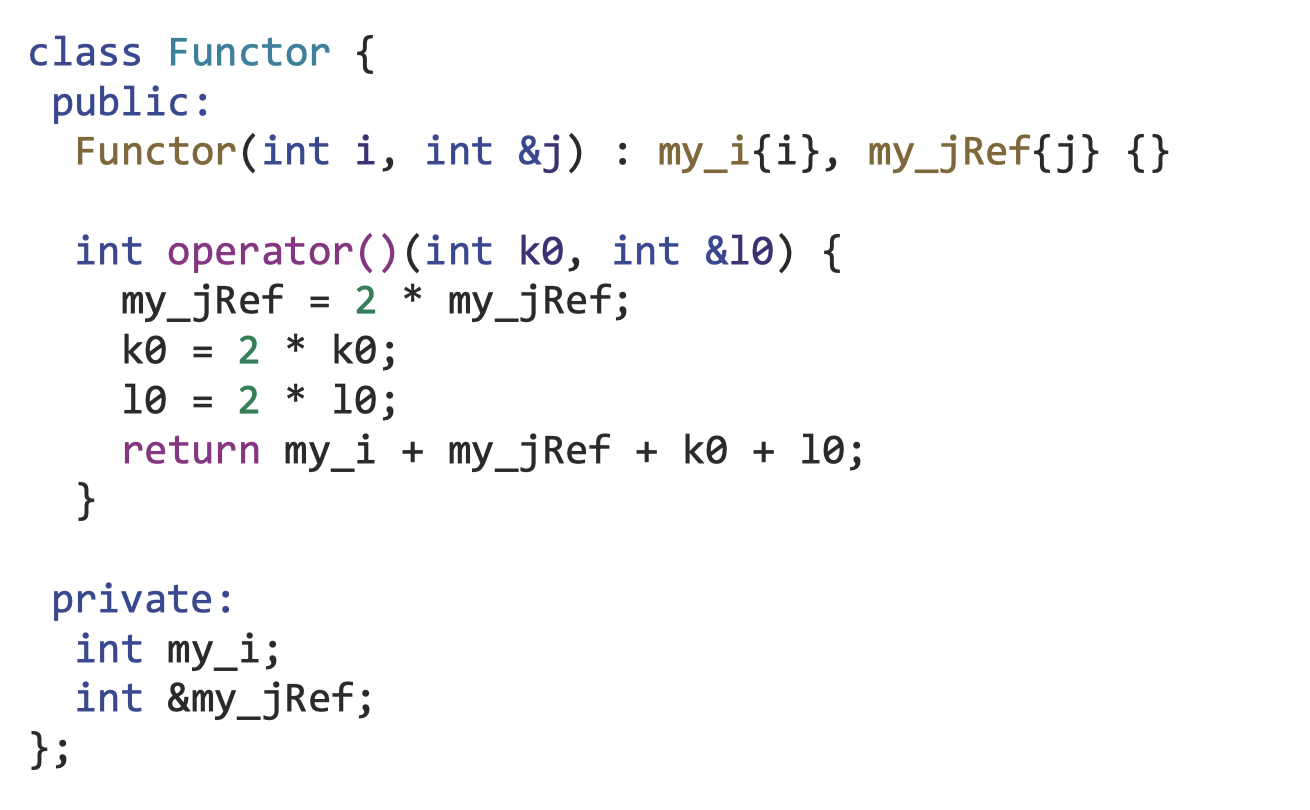
\includegraphics[width=0.9\textwidth]{figs/F1.6.png}
	\caption{\textit{函数对象而不是 lambda 表达式(第 10 章中有更多介绍)。}}
\end{figure}

我们可以将 lambda 表达式视为函数对象的实例,但编译器为我们创建了类定义。 
例如,我们在前面的示例中使用的 lambda 表达式类似于图 1-6 中所示的类实例。 
无论我们在哪里使用 C++ lambda 表达式,都可以将其替换为函数对象的实例,如图 1-6 所示。

每当我们定义一个函数对象时,我们都需要给它指定一个名称(图 1-6 中的 Functor)。 
内联表达的 Lambda 表达式(如图 1-4 所示)是匿名的,因为它们不需要名称。

\subsubsection{功能可移植性和性能可移植性}
可移植性是将 C++ 与 SYCL 结合使用的一个关键目标; 然而,没有什么可以保证这一点。 
语言和编译器所能做的就是让我们在需要时更容易在应用程序中实现可移植性。 
确实,更高级别(更抽象)的编程(例如特定于领域的语言、库和框架)可以提供更多的可移植性,
很大程度上是因为它们允许较少的规范性编程。 
由于我们在本书中重点关注 C++ 中的数据并行编程,因此我们假设希望拥有更多的控制权,
并因此承担更多的责任来理解我们的编码如何影响可移植性。

可移植性是一个复杂的主题,包括功能可移植性和性能可移植性的概念。 
凭借功能的可移植性,我们希望我们的程序能够在各种平台上同等地编译和运行。 
凭借性能可移植性,我们希望我们的程序能够在各种平台上获得合理的性能。 
虽然这是一个相当软的定义,但反过来可能会更清楚——我们不想编写一个在一个平台上运行超快的程序,
却发现它在另一个平台上运行得慢得不合理。 事实上,我们希望它能够充分利用其运行的任何平台。 
鉴于异构系统中的设备种类繁多,性能可移植性需要我们作为程序员付出巨大的努力。

幸运的是,SYCL 定义了一种可以提高性能可移植性的编码方法。 首先,通用Kernel可以在任何地方运行。 
在有限的情况下,这可能就足够了。 更常见的是,可能会为不同类型的设备编写重要Kernel的多个版本。 
具体来说,Kernel可能具有通用 GPU 和通用 CPU 版本。 有时,我们可能希望将Kernel专门用于特定设备,例如特定 GPU。 
当这种情况发生时,我们可以编写多个版本,并将每个版本专门用于不同的 GPU 模型。 
或者我们可以参数化一个版本以使用 GPU 的属性来修改 GPU Kernel的运行方式以适应现有的 GPU。

虽然我们作为程序员自己负责设计有效的性能可移植性计划,但 SYCL 定义了允许我们实施计划的构造。 
如前所述,可以通过从适用于所有设备的Kernel开始,然后根据需要逐步引入其他更专业的Kernel版本来对功能进行分层。 
这听起来不错,但程序的整体流程也会产生深远的影响,因为数据移动和整体算法选择很重要。 
了解这一点可以让我们深入了解为什么没有人应该声称带有 SYCL(或其他编程解决方案)的 C++ 解决了性能可移植性。 
然而,它是我们工具包中的一个工具,可以帮助我们应对这些挑战。


\subsection{并发与并行}
并发和并行这两个术语不一定是等价的,尽管它们有时会被误解。 
由于不同来源很少就相同的定义达成一致,因此对这些术语的任何讨论都变得更加复杂。

请考虑《Sun Microsystems 多线程编程指南》中的这些定义:
\footnote{The authors are fans of this programming guide’s coverage of the fundamentals that never go away. It is online at docs.oracle.com/cd/ E19253-01/816-5137/816-5137.pdf.}

\begin{itemize}
	\item 并发:当至少有两个线程正在进行时存在的条件

	\item 并行性:两个线程同时执行时存在的条件
\end{itemize}

为了充分理解这些概念之间的差异,我们需要对这里重要的内容有一个直观的理解。 
以下观察可以帮助我们获得这种理解:

\begin{itemize}
	\item 可以伪造同时执行:即使没有硬件支持一次执行多件事情,软件也可以通过多路复用来伪造同时执行多件事情。 
		多路复用是没有并行性的并发的一个很好的例子。

	\item 硬件资源是有限的:硬件永远不会无限“宽”,因为硬件始终具有有限数量的执行资源(例如处理器、Kernel、执行单元)。 
	当硬件可以使用专用资源执行每个线程时,我们就拥有并发性和并行性。
\end{itemize}

当我们作为程序员说“同时执行 X、Y 和 Z”时,我们通常并不真正关心硬件是否提供并发性或并行性。 
我们可能不希望我们的程序(包含三个任务)无法在只能同时运行其中两个任务的机器上启动。 
我们希望并行处理尽可能多的任务,重复地逐步执行批量任务,直到它们全部完成。

但有时,我们确实关心。 我们思维中的错误可能会产生灾难性的影响(例如“死锁”)。 
想象一下,我们对上一段的示例进行了修改,使得任务(X、Y 或 Z)执行的最后一件事是“等待所有任务完成”。 
如果任务数量永远不会超过硬件的限制,我们的程序就会运行得很好。 
但是,如果我们将任务分成批次,那么第一批中的任务将永远等待。 不幸的是,这意味着我们的应用程序永远不会完成。

这是一个很容易犯的常见错误,这就是我们强调这些概念的原因。 
即使是专家程序员也必须集中精力避免这种情况,而且我们都发现,当我们在思考中遗漏某些内容时,我们将需要调试问题。 
这些概念并不简单,C++ 规范包含一个很长的部分,详细说明了保证线程取得进展的精确条件。 
在这个介绍性部分中,我们所能做的就是强调尽可能多地理解这些概念的重要性。

直观地掌握这些概念对于异构和加速系统的有效编程非常重要。 我们都需要给自己时间来获得这种直觉——它不会一下子发生。

\subsection{总结}
本章提供了通过 SYCL 理解 C++ 所需的术语,并复习了对 SYCL 至关重要的并行编程和 C++ 的关键方面。 
第 2、3 和 4 章详细介绍了使用 C++ 和 SYCL 进行数据并行编程的三个关键:
需要为设备提供工作(发送代码以在其上运行)、提供数据(发送数据以在其上使用) ),并且有编写代码的方法(Kernel)。